\section{Crawling Process}

The first step consisted in the implementation of a crawler in order to retrieve tweets from Twitter. For the assigned task we decided to opt for a focused crawling approach. A list of user has been selected for each topic of interest and for each user the crawler retrieved at most \numprint{3200} tweets (which is the upper limit imposed by Twitter APIs). Each list has been chosen using the Twitter's \textit{lists} feature to find relevant profiles which tweets about the given topic.
The crawler has been implemented in Python using the \verb|tweepy| package which wraps Twitter's official APIs using a PostgreSQL database to persist the data and the \verb|multiprocessing| module to speed up the crawling process. The first phase consists in retrieving all the information regarding the selected users and storing them in the database. The second step is where the actual crawling of the tweets takes place. 
The crawler has been designed as a concurrent system: each process selects a new user to be processed from a shared queue containing all the users whose tweets need to be saved, then retrieves all the available tweets and after a basic pre-processing stores them in the database.

\begin{figure}[!h]
    \centering
    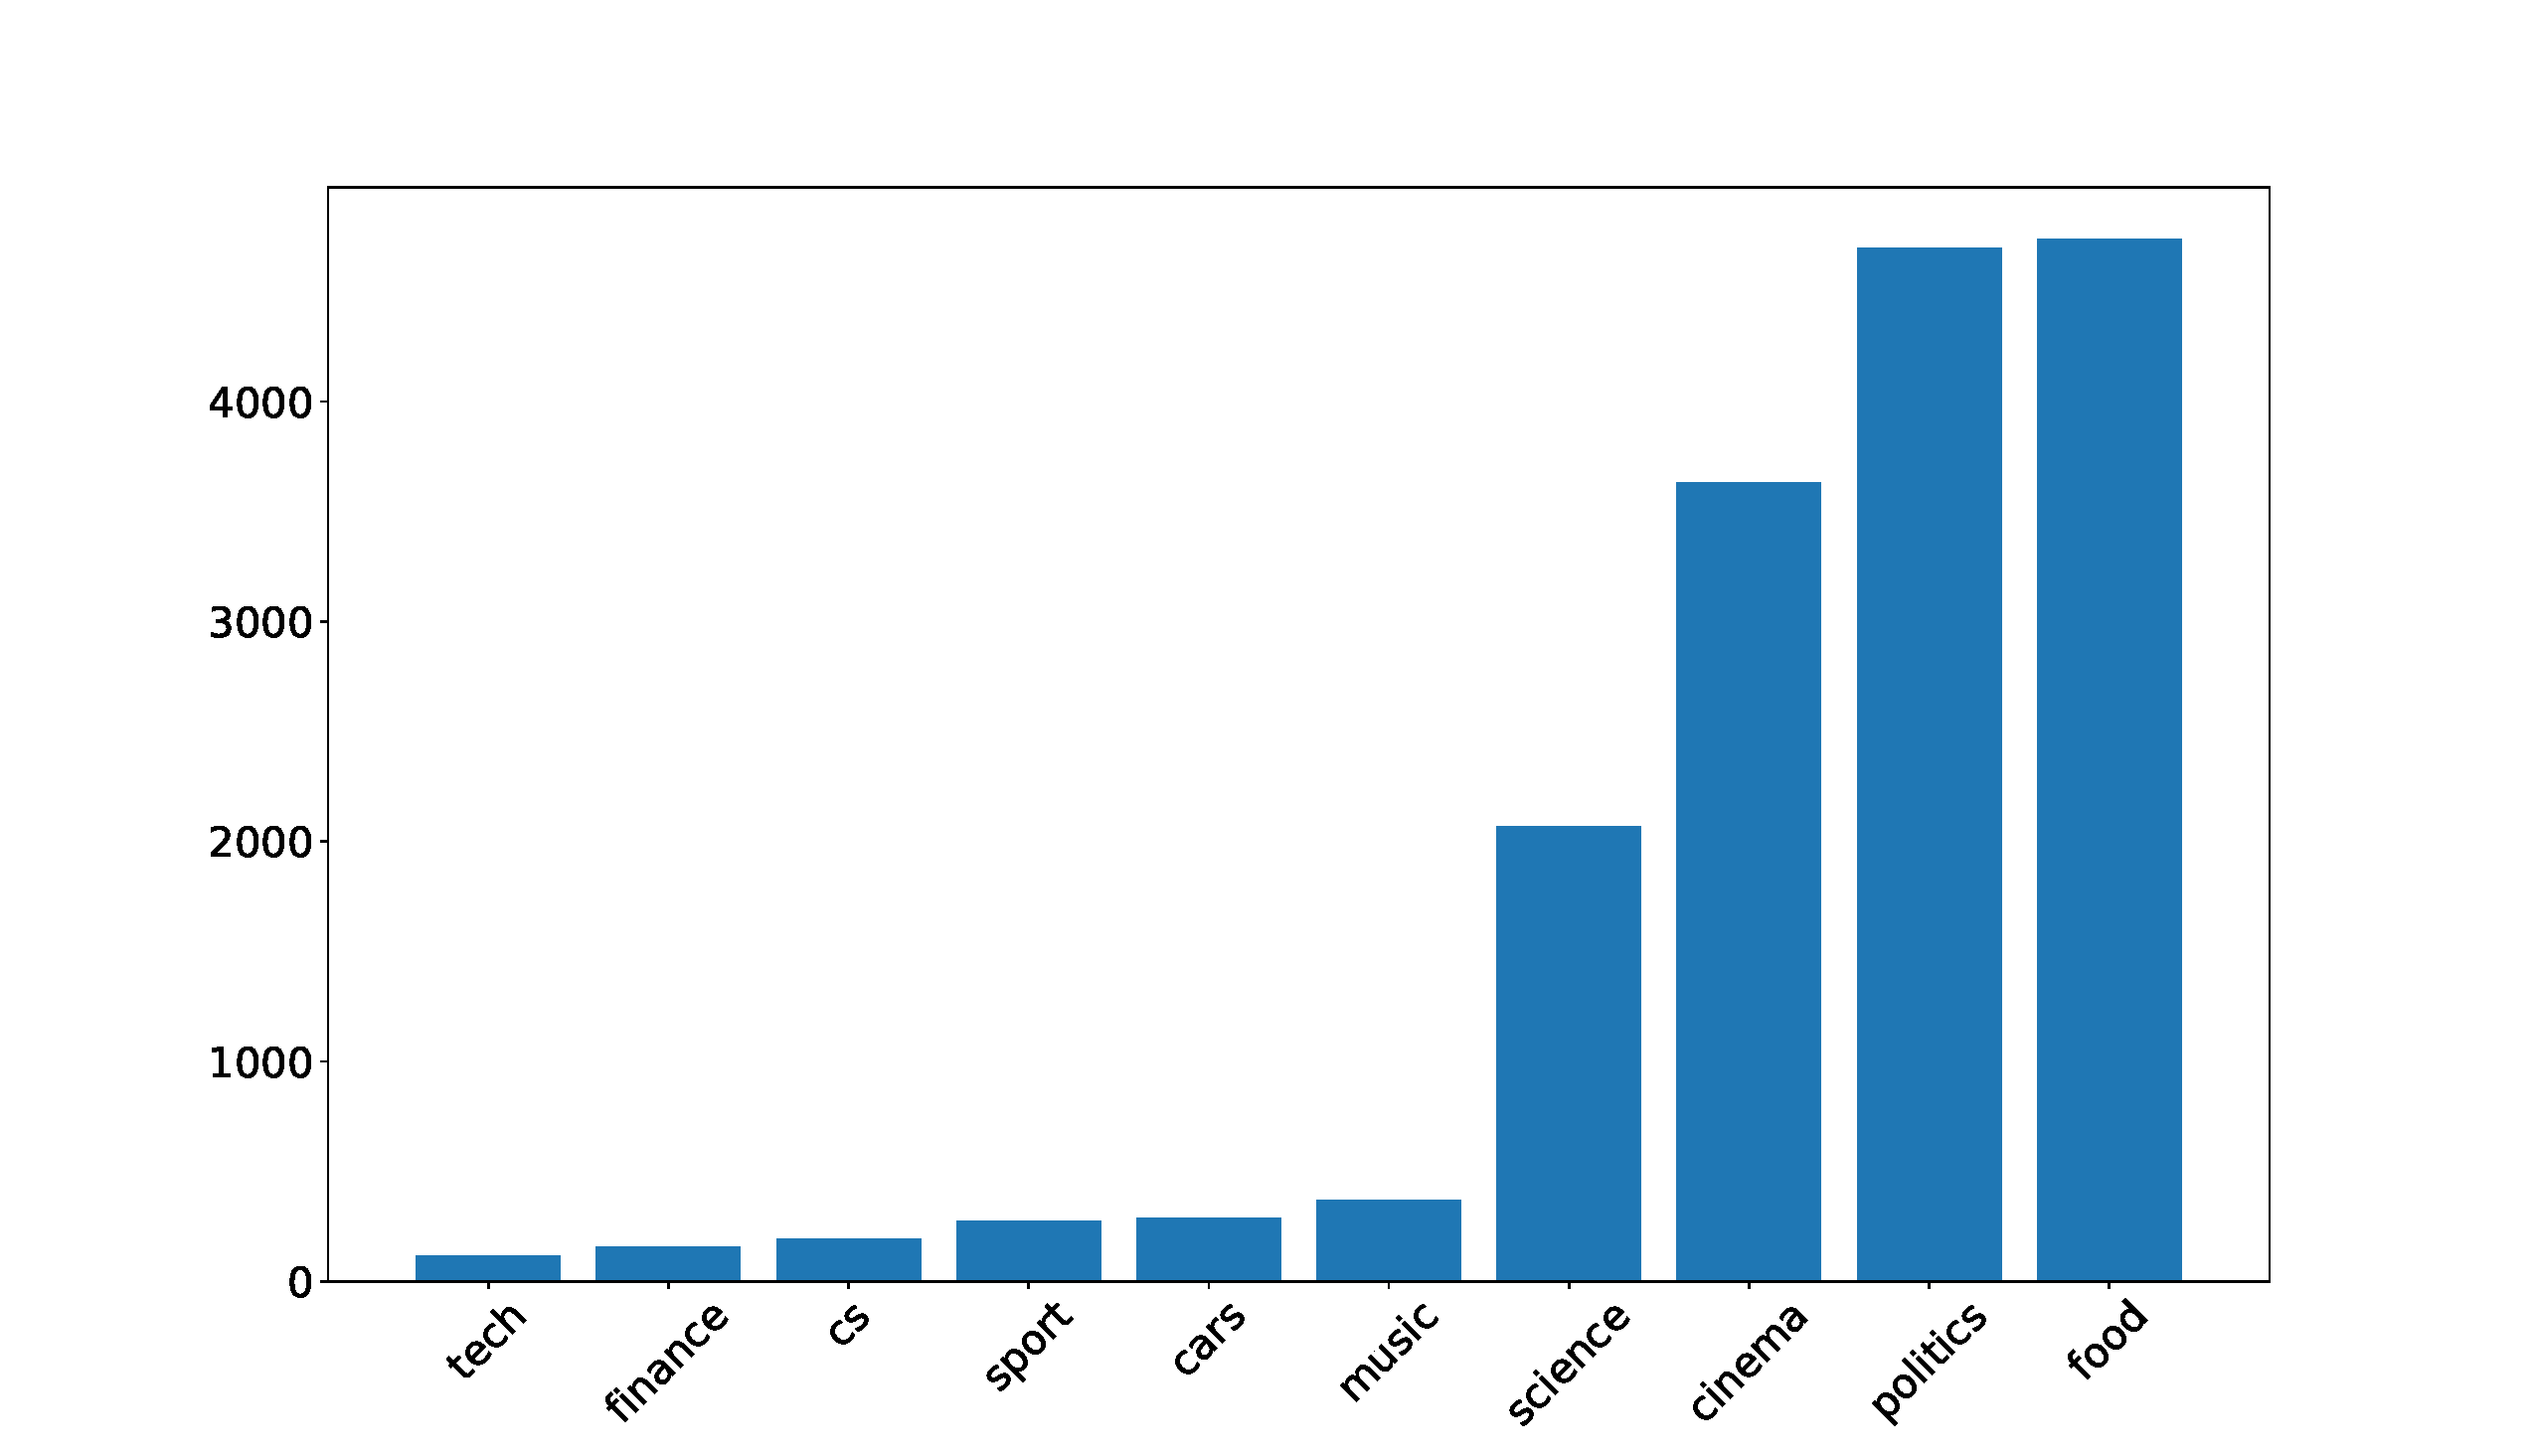
\includegraphics[width=1\textwidth]{topics.eps}
    \caption{Number of users for each topic}
    \label{fig:users-distribution}
\end{figure}


\subsection{Dataset}

In total \numprint{35699286} tweets have been crawled from \numprint{16185} different twitter users after discarding all the tweets in a language different than english (based on the \verb|lang| field in the JSON). The crawler stored, for each user, its followers, the topic to which the user belongs and the raw JSON returned by Twitter's APIs. In the same way, for each tweet its author and the corresponding raw JSON has been stored.

In figure \ref{fig:users-distribution} the distribution of users for each topic taken into account.
It can be seen that the number of users is not uniformly distributed among topics and four of them have significantly more users. We decided not to use the same number of users in each topic since in the real world - not necessarily for the same categories used in this project - we expect that there are topics more discussed than others.

\begin{table}[ht]
	\scriptsize
	\centering	
	\begin{tabularx}{0.24\textwidth}{r r}		
		%\toprule		
		\textbf{Percentile} & \textbf{Follower}\\				
		\midrule				
			5    & 226                  \\
			10   & 391                  \\
			20   & 746                  \\
			30   & \numprint{1210}      \\
			40   & \numprint{1879}      \\
			50   & \numprint{2954}      \\
			60   & \numprint{4625}      \\
			70   & \numprint{7851}      \\
			80   & \numprint{14563}     \\
			90   & \numprint{39785}     \\
			95   & \numprint{105922}    \\
			97   & \numprint{231844}    \\
			99   & \numprint{1262254}   \\
			99.5 & \numprint{3120360}   \\
			100  & \numprint{104683236} \\
		\vspace{5pt}
		%\bottomrule \\
	\end{tabularx}
	\captionof{table}{} 
	\label{tab:percentile_follower} 	
\end{table}
\noindent
In Table \ref{tab:percentile_follower} instead are reported the percentiles of the followers. It can be seen that almost 30\% has less than \numprint{1000} followers and about 5\% of the most followed users have more than 100 000 followers with the majority of the others having between \numprint{10000} and \numprint{40000} followers.
